\documentclass[11pt]{scrartcl}
\usepackage{graphicx}
\graphicspath{{./}}
\usepackage[sexy]{evan}
\usepackage[normalem]{ulem}
\usepackage{hyperref}
\usepackage{mathtools}
\hypersetup{
    colorlinks=true,
    linkcolor=blue,
    filecolor=magenta,      
    urlcolor=cyan,
    pdftitle={Overleaf Example},
    pdfpagemode=FullScreen,
    }

\renewcommand{\dangle}{\measuredangle}

\renewcommand{\baselinestretch}{1.5}

\addtolength{\oddsidemargin}{-0.4in}
\addtolength{\evensidemargin}{-0.4in}
\addtolength{\textwidth}{0.8in}
% \addtolength{\topmargin}{-0.2in}
% \addtolength{\textheight}{1in} 


\setlength{\parindent}{0pt}

\usepackage{pgfplots}
\pgfplotsset{compat=1.15}
\usepackage{mathrsfs}
\usetikzlibrary{arrows}

\title{Seleksi SMAN 5 Bekasi}
\author{105 menit}
\date{Sabtu, 11 Februari 2023}

\begin{document}

\maketitle
\section{Isian Singkat Bagian Pertama}
Setiap nomor bernilai 1,5 jika benar, 0 jika kosong atau salah. \textbf{Tulis hasil akhirnya saja}
\begin{enumerate}
\item Ada berapa banyak bilangan 4-angka (digit) yang semua angkanya genap dan bukan merupakan kelipatan 2003?

\item Sebuah kelas terdiri dari 40 siswa. Diantaranya, 20 siswa menyukai pelajaran Matematika, 15 orang menyukai pelajaran Biologi, 15 orang menyukai pelajaran Bahasa Inggris dan lima orang menyukai ketiganya. Banyaknya siswa yang menyukai sedikitnya satu dari ketiga pelajaran tersebut adalah ?

\item Di dalam suatu lingkaran $L_1$ yang berjari-jari 1 dan berpusat di titik $(0,0)$, digambar suatu lingkaran $L_2$ yang bersinggungan dengan lingkaran $L_1$ , sumbu-x dan sumbu-y positif. Panjang jari-jari
lingkaran $L_2$ adalah \dots

\item Hari ini usiaku $\tfrac{1}{3}$ kali usia ayahku. Lima tahun yang lalu, usiaku $\tfrac{1}{4}$ kali usia ayahku pada waktu itu. Berapakah usiaku sekarang ?
\end{enumerate}

\newpage
\section{Isian Singkat Bagian Kedua}
Setiap nomor bernilai 3,5 jika benar, 0 jika kosong atau salah. \textbf{Tulis hasil akhirnya saja}

\begin{enumerate}
    \item Misalkan suatu fungsi $f: \RR-\{0\} \to \RR$ memenuhi
\begin{align*}
    f\left(\dfrac{1}{x}\right)+\dfrac{1}{x}f\left(-x\right)=2x
\end{align*}
untuk setiap bilangan real $x \neq 0$. Berapakah nilai $f(2)$? 

    \item Berapakah sisa pembagian $1\cdot 1!+2 \cdot 2! + \dots + 100 \cdot 100!$ oleh 101?

    \item Berapakah banyaknya cara memilih tiga bilangan berbeda sehingga tidak ada dua bilangan yang berurutan, jika bilangan-bilangan tersebut dipilih dari himpunan $\{1, 2, 3,\dots, 9, 10 \}$ ?

    \item Diberikan segitiga $ABC$ siku-siku di $A$, titik $D$ pada $AC$ dan titik $F$ pada $BC$. Jika $AF \perp BC$ dan $BD=DC=FC=1$, maka $AC= \dots$
\end{enumerate}


\newpage
\section{Esai}
Setiap nomor bernilai bilangan bulat dari 0 sampai 8. \textbf{Tulis dengan cara atau argumentasinya}
\begin{enumerate}
    \item Jika hasil  perkalian
\begin{align*}
    \left(1-\dfrac{1}{2^2}\right)\left(1-\dfrac{1}{3^2}\right)\left(1-\dfrac{1}{4^2}\right)\dots \left(1-\dfrac{1}{2023^2}\right) = \dfrac{a}{b}
\end{align*}
dimana $a$ dan $b$ adalah bilangan asli yang saling relatif prima, hitunglah nilai $a+b$. Jelaskan.

\item Carilah dua digit terakhir dari $17^{83}$.

\item Misalkan ada 5 orang siswa yang duduk mengelilingi sebuah meja bundar. Lalu, Anya dan Sagiri datang dan akan duduk mengelilingi meja bundar tersebut. Namun, karena Sagiri pemalu, ia hanya ingin duduk tepat disebelah Anya saja. Berapa banyak kemungkinan tempat duduk yang dapat terjadi pada ketujuh orang tersebut? Jelaskan.

\item Diberikan tiga bilangan real positif $x,y,$ dan $z$ yang semuanya berbeda. Jika 
$$\dfrac{y}{x-z}=\dfrac{x+y}{z}=\dfrac{x}{y}.$$ Berapakah nilai $\dfrac{x}{y}$? Jelaskan.

\item Pada sebuah segitiga $ABE$, titik $C$ terletak pada segmen $AE$ dan $D$ pada $BE$ sedemikian sehingga $CD \parallel AB$. Selanjutnya, titik $F$ di garis $AD$ sedemikian sehingga $EF \parallel AB$. Jika $AB=5$, $EF=3$, berapakah panjang $CD$? Jelaskan.
\begin{center}
    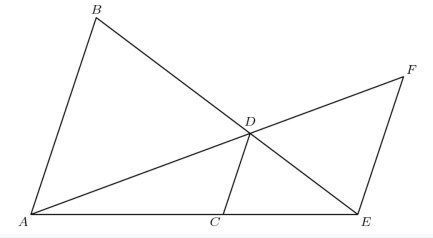
\includegraphics[scale=0.8]{soal tes geom.PNG}
\end{center}

% \item Diberikan segitiga lancip $ABC$. Titik-titik $D,E,F$ berturut-turut berada di garis $BC,CA,AB$ sedemikian sehingga $AD \perp BC$, $BE \perp CA$, dan $CF \perp AB$. Garis $AD$ dan $BE$ bertemu di titik $H$,
% \begin{enumerate}[a)]
%     \item Buktikan bahwa $BEHF$ siklis.
%     \item Tunjukkan bahwa $BH$ merupakan diameter lingkaran luar segiempat $BEHF$.
% \end{enumerate}
\end{enumerate}
\end{document}
